\chapter{Contribution}
In this chapter ..

In the following sections "Observable" is used to denote an actual RxJS Observable and also as a placeholder for any Reactive entity from RxJS or BaconJS in lack of a better term.

\section{Advancing the User Interface}
The User Interface (UI) is an important part of every application. A good UI helps the user focus on the task at hand by displaying the necessary information required for that task. For a Website this task may simply be to find gather information about the subject of the Website itself. An IDE usually provides many tools the user can use and reduce the manual work of the user by automating some steps of the development process. There are many factors that need to be taken into account when developing a new UI or changing an existing one. A UI should normally be designed to match the special use-cases the application was designed for while also keeping some familiar elements to guide the user. The main reason to keep a somewhat familiar look or have a certain part of the UI match what the user expects and knows from other applications in his domain, is that the user already knowns how to interact with familiar elements and does not have to learn how to use them from scratch. It is also important to consider some of the characteristics of human cognition. To explain them all in detail is beyond the scope of this thesis. To solve this type of problems if a main target of the Interactive Graphics Systems Group (GRIS) at TU-Darmstadt and many other groups world wide are working in this field. In the following paragraph we examine the changes to the UI of CRI we implemented in this thesis and the reasoning behind these changes.
  
\textbf{Reducing the cognitive load on the user}
The main goal of the changes to the UI we implemented in this thesis is to reduce the cognitive load on the user. If the user has to concentrate and search for information they need to achieve their task and not having them presented in an easy to find and understand manor, half of his attention is already occupied. It can not be used to work on the task and achieve their actual goal.

The first change we introduced to reduce the cognitive load on the user is to move some input elements to a menu that is displayed at the top of the CRI's UI. Nearly every desktop application and many Websites (e.g. http://reactivex.io/rxjs/, Windows File Explorer, Eclipse, Microsoft Paint, Adobe PDF Reader and many more) use a menu at the top of the UI. This adds structure and also removes many buttons from the normal working space which can then be used to display more relevant information. The user knows that the buttons are in the menu and searches though it on demand. The buttons hidden in the menu bar do not require space or attention by the user at other times, except for the space required by the menu itself. We examined our own usage frequency, how often we use a certain input element, and estimated the tasks that include the input element to determine which elements should be part of the main UI and which should be hidden in a menu (or closeable panel for inputs other than buttons). We found that we rarely used the \emph{Reset}, \emph{Download} and \emph{Pause/Resume} buttons. The latter was used most among them and since CRI does not actually have loads of buttons yet, we decided to place it directly in the menu bar instead of moving it into the sub menu used for the other rarely used buttons. The \emph{Pause/Resume} button is also the only one of those buttons used in a normal workflow, i.e. in the special case of working with Rapidly updated Observables (see section \ref{sec:RapidlyUpdatedObservables}) it is used regularly to counter performance issues or focus on a specific part of the execution.  %TODO: maybe add screenshot of menu
The other buttons of the UI are part of a specific feature of CRI and can not be moved away from other elements that belong to the features. These features from left top to bottom right are the Instrumented Files list, History Queries and the navigation through the results, Reactive Breakpoints, Search, History Navigation and the Dependency Graph. The Dependency Graph and History Navigation are closely tied together and represent the main part of CRI. They are the working area where the focus of the UI should be. The other features are complementary to them support the user ins examining their content. Although CRI can be used effectively without History Queries and Reactive Breakpoints they can help the user in almost any task. Reactive Breakpoints may even be mandatory to discover some issues with an application that otherwise could not be detected without a much greater effort (similar to normal Breakpoints in traditional IDEs). While the Dependency Graph with its History is just another way to provide an abstract representation of Observables and Dependencies then the Marble Diagrams used in RxFiddle, Reactive Breakpoints are currently exclusive to CRI. In conclusion, History Queries and Reactive Breakpoints should be a permanent part of the UI, therefore we decided to keep them where they were positioned in CRI2 - above the History Navigation. The Search feature is not as important in most tasks. The highlighting of a specific node, its Dependencies or Dependents is only useful for applications with large Dependency Graphs. Small graphs can easily be searched for the required information manually with one look. Therefore the Search feature could be moved to a closeable panel that is only opened on demand. The search implemented in most IDEs opens when the user presses CTRL F or clicks the search button in the menu. The reason we did not move the feature to a closeable panel yet is simply that the area of the UI where the History Query and Reactive Breakpoints input elements are placed provides enough space (with standard screen resolutions sizes for desktop computers) to keep the Search there as well. With the current UI the space would otherwise be empty. However as soon as these parts of the UI change or another feature is introduced, the Search should be moved to a closeable panel. The remaining feature is the Instrumented Files list. It is used as a scoping feature to select which files should be instrumented. For small to medium sized applications the list of files will normally include all relevant JS files and will not be changed at all. It is therefore reasonable to move it from the main UI to free the space that could then be used to increase the size of the Dependency Graph canvas. After examining the outcome of this change we found however, that in case the user switches to another application that requires other files to be instrumented or forgot to include a JS file in the list, it can be really difficult to detect the reason why the Dependency Graph is not showing the expected result. If the Instrument Files list is moved from the main UI, the user may loose track of the fact that not all JS files are automatically instrumented or, if they decided to instrument only a subset of JS files as a filtering measure, that the >filter< is still in place. It is also easier for new users to comprehend the need to select files for instrumentation if the list is part of the main UI. This could be mitigated by adding a dialog informing the user at the first start of CRI, but for this reason in addition to the reasons mentioned above we decided the benefits outweigh the downside of a small part of the UI being occupied by a rarely changed input. Therefore we kept the Instrument Files list at the top of the UI and also added a red border around the text input as an validation error in case the list is empty to help make new users aware of the missing input.

To further decrease the cognitive load when working with CRI, we removed any text from nodes and their tooltips that do not carry any value. The less text there is on the UI, the less as user has to read to find the information that they require. This is most significant for the \emph{Method} field in the tooltips since most Observables do not correspond to a method and the field therefore is empty for most nodes. The \emph{Value} field is usually set, but if there is no value, there is no need to keep the label for the field. The same information is available to the user if the label for \emph{Value} is simply omitted in that case.
It is however important to display values that explicitly denote an \emph{empty} value like \emph{undefined}, \emph{null}, or -1 (for a value that carries positive numbers if it is set). The \emph{Name} field is also not set for every node. Figure \ref{fig:Nodes} shows an example of nodes from CRI2 with all field as well as nodes from the current version.

\begin{figure}[!h]
	\centering
	\subfloat[CRI version 2.0]{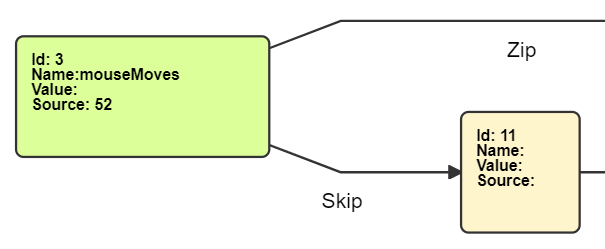
\includegraphics[width=0.4\textwidth]{gfx/NodesCRI2.png}\label{fig:NodesCRI2}}
	\hfill
	\subfloat[CRI version 3.0]{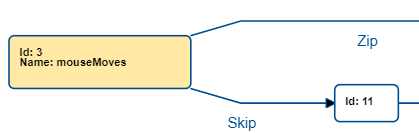
\includegraphics[width=0.4\textwidth]{gfx/NodesCRI3.png}\label{fig:NodesCRI3}}
	\caption{A sample of nodes before and after the changes introduced by this thesis.}
	\label{fig:Nodes}
\end{figure}
%TODO: casing of \emph{Named} node and dependency
Another important aspect to consider is if to display a field on the node directly or in the tooltip. The same principle that applies to general elements of the UI applies here as well. Only values that are necessary to always have present without the need to open every tooltip should be displayed as part of the nodes. We evaluated for each field where it should be located regarding this criteria. The \emph{Name} is important to identify relevant nodes, including those depending or dependent on a \emph{Named} node. The \emph{Id} is required to add Reactive Breakpoints and to identify nodes without a name from one step to another in case the nodes are repositioned due to a new edge being added. The \emph{Value} is normally the property at which developers can see if the JS code of the application works as intended. E.g. an Observable is expected to have a specific value at some point in the execution. The developer can also observe a value passing along the chain of dependencies. For these reason the fields \emph{Name}, \emph{Id} and \emph{Value} should be always displayed, as long as they have a value, as part of the node.
The \emph{Type} should be hidden in the tooltip, because often what type of Observable the framework uses internally does not matter to the developer. E.g. in most scenarios for RxJS there is not difference between a FromEventObservable and a basic Observable. The information should however, be still present in the tooltip and not omitted completely, because some types of Observables do behave differently than others e.g. RxJS Subject vs Observable. The source code position labeled \emph{Source} is also just used in few special tasks. On example is the user wanting to find the source code corresponding to a node in the graph to modify that code or inspect it further. The \emph{Source} should therefore be displayed in the tooltip rather the nodes themselves. The field \emph{Number of Updates} was introduces by this thesis as a way to detect bottlenecks and help identify nodes that cause the generation of a huge amount of steps through excessive value updates in CRI. It is based on the Time Profiling feature of the Reactive Inspector \cite{ReactiveInspector}, but for now only provides the total number of updates on a node instead of detailed timing and value evaluation information. It is only useful for the purposes mentioned above and therefore should not be displayed on the nodes themselves.

An important cognitive task that a user has to do often while using CRI is to track changes between steps in the Dependency Graph History. To track these changes is necessary to understand how the graph is constructed or to track value updates traveling along a chain of dependent Observables. It is however not always trivial since the rendering engine \emph{D3.js} \cite{D3JS} used by CRI sometimes moves nodes and edges around to better fit the available space. To help the user with this task, the previous version of CRI already highlighted the nodes that were changed for each step in which a node was changed. We extended this feature to also highlight edges that were updated or added to further decrease the manual searching process. Another feature we added to the UI is a button that hides the tool section of the UI - everything except the menu, History Navigation and Dependency Graph - to allow the user to reduce distractions and free up additional space if they want to focus on the manual examination of the graph and its History. The button is located at the top right corner and has a small arrow icon instead of a text label to reduce its required space in the UI. The option to hide the tool section is especially useful when working with a small screen or a big Dependency Graph. Another button we added to the UI, as part of the menu, was a button to reload the inspected page and therefore the Dependency Graph as well. We discovered that reloading, was already part of the usual workflow by pressing CTRL F5 and decided to add a button that allows user to achieve this without being aware of the short cut. An example workflow in which reload would be used is to create a breakpoint for \emph{dependencyCreated} or \emph{nodeCreated}, and then reloading the application to actually hit the breakpoint.
As figure \ref{fig:Nodes} shows, we also change the colors used in the CRI UI. The node that was changed in the currently viewed step was highlighted by using a red border in the previous version of CRI. The color red is a signal color normally used to show that immediate attention is required or to show that an error has occurred. In traffic signs and lights the color red is used to signal cars to stop or to be aware of dangers. Therefore we decided to remove it from the normal workflow of CRI. Highlighting the current node is important for the user to immediately identify the change, but it does not require the users full attention the whole time. It also neither represents an error, therefore the increased cognitive load on the user is unnecessarily. The combination of red and green (\emph{Named} nodes) may also be problematic for some users with vision deficiency, although as the green is a very bright shaded they should still be able to distinguishable the border on a highlighted \emph{Named} node. Because of these reasons we decided to use blue with light orange as the highlighting that has less contrast between the two shades, but still enough to not void the highlighting. To this purpose we chose a shade of blue and selected the colors for nodes, edges and highlighting from suggestions provided by a color scheme designer \cite{Paletton}. We chose to keep the text color black, because it is the most used color for text in general and is easy to read on most colored backgrounds. The nodes that do not correspond to a named variable were left without a background to further reduce the cognitive load. The brain is trained to ignore empty spaces therefore making the text and named nodes appear more important.

Another change we introduced to the UI of CRI was the automatic reloading of the graph if the Instrumented Files list changes. This does not reduce the cognitive load on the user, but removes a redundant click on the reload button. It is not very useful to change the list of instrumented files without restarting the inspected application and the recording. If the application is not reloaded automatically it may also confuse the user that their change does not have an immediate effect. 
	
\section{Connecting abstract graph with JavaScript code}
Nodes in the Dependency Graph that correspond to Observables that are directly assigned to variables provide developers with some form of context. A \emph{Named} node can be used as an anchor to identify the node itself as well as other nodes up and down the chain of dependencies. It helps the user to separate parts of the Dependency Graph that are relevant for the piece of code they want to examine and parts that are currently not relevant. Without any orientation it is very hard to interpret a shown Dependency Graph. The user can still try to identify nodes by their values or the values of their neighbors, but these values can be missing at certain stages of the application. This all boils down to the issue of connecting the abstract representation of the applications Observables provided by the Dependency Graph with the actual JS source code responsible for those Observables. If an error is detected by examining nodes in the Dependency Graph, the user still has to track down which lines of code are responsible for the issue in order to change them. As mentioned above, \emph{Named} nodes solve this issue in a way, but not all Observables created during runtime are assigned to variables. In fact, even if possible, this is not at all desirable. To the result of each function in a chain of functions to a variable negates most of the benefits of using chained functions in the first place. If the variables are not used by multiple lines of code and are just introduced to support the debugging tool, most of all the disadvantages of \emph{do-debugging} apply as well. We therefore evaluated several possibilities to provide nodes that do not have a corresponding variable with additional details that help provide some context to the user. A very basic form of context was already present in the previous versions of CRI in form of the source code position information. This information was however, not very accurate in case of chained functions, because only the start of the source code position information provided by Jalangi was used. In case of chained functions the source code position actually spans a block that may consist of multiple lines of source code. In addition information provided did not contain the name of the JS file to which the position belongs. Another downside of this approach is that to look up the source code in another tool apart form CRI and switching back to CRI to check the position of the next node would be very cumbersome to execute for more than a few nodes. The developer should be able to easily switch between source code inspection and examining the Dependency Graph, because not all issues can be found in either of them when used alone. For example, if there is an issue in a lambda function, a user can not find this issue directly in the Dependency Graph. They can only see the result in node values that do not match the values they would expected with the original intention of the code in mind. The main difficulty to achieve this by showing actual source code instead of just the position information is JS code that is used during runtime is instrumented with Jalangi to enable a detailed analysis. Jalangi instrumented code is very hard to read as is shown in listing \ref{lst:Instrumented}.

\begin{lstlisting}[language=JavaScript, caption={Example of RxJS code.},label={lst:Instrumented}]
$sonWallet = J$.W(593, '$sonWallet', J$.F(585, J$.I(typeof $ === 'undefined' ? $ = J$.R(569, '$', undefined, true, true) : $ = J$.R(569, '$', $, true, true)), false)(J$.T(577, '#wallet-son', 21, false)), J$.I(typeof $sonWallet === 'undefined' ? undefined : $sonWallet), true, true);
$fatherWallet = J$.W(625, '$fatherWallet', J$.F(617, J$.I(typeof $ === 'undefined' ? $ = J$.R(601, '$', undefined, true, true) : $ = J$.R(601, '$', $, true, true)), false)(J$.T(609, '#wallet-father', 21, false)), J$.I(typeof $fatherWallet === 'undefined' ? undefined : $fatherWallet), true, true);
\end{lstlisting}

For example "J\$.W" signals the analysis engine that a write operation is executed when the function is called. This makes it unfeasible to directly show the instrumented code to the user. In addition to being very hard to read, the instrumentation of the source code is an implementation detail of CRI and should not be exposed. Additionally the code position retrieved from the Jalangi analysis corresponds to the position in the original source code without instrumentation. Note that the JS code that is used during runtime is also dynamically loaded and therefore can not be navigated to out of the box with Chrome DevTools navigation API. Although this is mitigated by adding "//\# sourceURL=" with a custom URL to the bottom of a script. Since this shows the Jalangi instrumented source code that is not useful for a normal user, we decided to tie this to a new option called \emph{CRI Developer Mode} that can be enabled in the options page of CRI. The different approaches discuss in the following section are designed to enable a user to use both the abstract representation and the source code in tandem.
	
\subsection{Evaluated possibilities of displaying source code}
\textbf{Using the \emph{chrome.debugger} API}\\
One possible option would be to use the \emph{chrome.debugger} API to open and navigate to the corresponding position of a node. It is easily possible navigating to a line number in a file, if the actual file URL, which can differ for dynamically loaded scripts due to many factors, is known. For the reasons explained above, navigating to the instrumented code is not desirable. A non-instrumented version seems to exist in Chrome's \emph{Source} windows as a dynamic script, but it is not actually used at runtime. This approach would provide the user with syntax highlighting through Chrome and other features like search with regular expressions. They could also inspect the whole code of the application, not just the piece of code corresponding to a single node if required. The downside of this approach is that the user needs to leave the UI of CRI to access the source information. For a single node this is not an issue, but it is really cumbersome to inspected the source information of multiple nodes, even if the navigation to the position is automated. It would not be possible to highlight the code block that corresponds to the inspected node, which would be especially useful for Observables corresponding to the middle of a block of chained functions. The start and end of the block would have to be manually searched for. Another downside that would most likely confuse the user, is that some features of Chrome's DevTools can be used but others will not work and there is no way for CRI to display this disparity. Due to the code shown to the user not actually being executed, all features specific to runtime interaction like breakpoints, direct code evaluation or watches will not be usable although a user familiar with Chrome's debugging capabilities will most likely expect them to work properly. A modification of this approach would be to display the code in another IDE than Chrome. As some modern IDE's provide a featured to navigate to a functions declaration (in WebStorm called "Go to declaration") which is more scalable than using a String based search for enterprise sized applications. Although this feature is not available in Chrome, having the user install another IDE and use that in parallel with Chrome will increase the dependencies of CRI and the development effort coupled with that dependency while still suffering from all the downsides of this approach explained above.\\
\textbf{Using an integrated lightweight IDE}\\
Another possibility would be to use a file viewer that is opened for example as a closable panel to show the full source code. Depending on the implementation this approach can provide full customization of code presentation to the user. In theory, advanced syntax highlighting (syntax highlighting based on the usage and structure of functions like WebStorm does to detect >classes<) could be applied. It would also be possible to highlight Observables in the source code while the user hovers over the in the Dependency Graph or even permanently coloring the source code based on the abstract representation. The main problem of this approach is the development effort required to achieve a viable implementation. There is no library available, that we are aware of, that provides the needed functionality and customization options. To develop such a library ourselves would require nearly the same amount of work needed to develop a traditional IDE for JS since it basically would be a lightweight JS IDE displayed in a panel of CRI. Another issue with this solution in addition to the required development effort is that nodes that are close in the Dependency Graph, because they share a dependency do not necessarily correspond to code that is located in close proximity of one another. The code may even be split over several JS files in extreme cases which would require additional view options by any lightweight IDE apart from just showing one JS file.\\ %TODO: search for 'web'
\textbf{Mirroring interactions to a non-instrumented copy of the application}\\
An approach that is possible in theory, but will not withstand a detailed evaluation would be to mirror any interaction to the inspected application to another version of it. The idea is to have one application with instrumented JS files, and one where the JS files are not instrumented. This would enable CRI to use another approach like using the \emph{chrome.debugger} API to display the actual source code used at runtime while retrieving analysis data from the instrumented mirror application. It would enable the user to use every feature of Chrome or another IDE when debugging JS. The problems introduced by copying the entire application and mirroring any interaction to it go, however, far beyond the doubled resource consumption. One mayor issue is the actual recording of user interactions to the original application. There are many tools like Katalong Studio \cite{Katalon} using Selenium \cite{Selenium} that can be used to record and replay interactions to a Web application. These tools are often used to automate the testing of Web applications. Most of these tools are therefore designed to ignored certain aspects of interactions like positioning of elements to make the tests more robust against small changes. Although there are some tools that use pixel positions to record and replay interactions. We could, however find not one tool that records mouse movements and replays them exactly. It would be possible to develop a solution oneself, but the mentioned tools solve many issues like always replaying with the exact same screen resolution that is especially important if the layout of the applications UI reacts to different screen resolutions. Another issue with replaying interactions to the copied Website are security restrictions imposed by Chrome (and other modern browser) itself. Chrome restricts some special interactions a user can execute to not be mimicked by a Web application of Chrome extensions to shield users from attackers that use a custom extension or Website to influence Web applications outside of their own domain. An example of these restricted interactions is the using of Chrome's Context Menu or the operating system's Clipboard. The reasoning to restrict both are similar and are due to the fact that these features can be used to breach boundaries otherwise monitored by Chrome itself or in case of the Clipboard by the operating system. Since these interactions can not be mimicked, it is impossible to replay them on the mirror Web application. This voids all other attempts to replay any other interaction, because the two applications will desynchronize. The danger of the two applications becoming desynchronized can also be created by Observables or JS code in general being time sensitive. For example an Observable or function that is scheduled to be executed or updated every few milliseconds and has any side effect like increasing a value by one every time the execution happens, would need to be mirror exactly to produce the same result on the mirrored application. This also includes any JS code that is execution order dependent. The same execution order must be maintained, which is especially hard for asynchronous code even though JS's runtime is event-based \cite{EventBasedJS} and does not actually execute code in parallel. In summary, any code dependent on the order of execution or anything timing related would have to be mimicked exactly to keep the mirror in sync with the original application, which can not be guaranteed for all possible applications in a normal environment. \\
\textbf{Source Code Tooltips}
	% Source Code Tooltips
		% - use tooltip that opens when CTRL is hold down on node that displays a snippet of the original code that contains the code corresponding to a node with surrounding lines of code. Or use CTRL click to open the snippet.
		% details in "Implemented Solution"
		%TODO: make sure there are not duplicates in Implemented Solution.
		% Pro: - precise highlighting of corresponding code possible
			% - serves as additional details for nodes, can help identify a node that has no name
			% - helps the user to find and remember a node without a name between multiple uses of the extension by other means than the id. The id may have changed due to changes to the previously executed code.
			% - fast to open/close and without leaving the extensions UI
		% Con: - if the chain of functions is to large, not all relevant code can be shown and in general big chains are hard to read.
			% - no search or other code inspection tools available for the code snippet -> the user would have to use an external tool and the line number for that. No breakpoints, though there are not that useful in reactive programming anyway as described in state of the art chapter.
			% - can not use existing syntax highlighting of chrome or an IDE. Implementing a own syntax highlighting would not be easy, because if just the small snippet is analysed all context relying highlighting will be lost. Basic keywords would be possible but with own implementation or third party library.
			% full code is not availabe for the user
			% the displayed code can not be examined with features like search - but they are short enough to be examined in a few seconds.
			
	\subsection{Implemented Solution - Source Code Tooltips}
	% display the origin  JS code of a node 
	% change tooltip to show the code if ctrl pressed while mouse enter or when already on element to speed up inspection of multiple nodes one after another
		% limited capabilities of used jalangi -> developed for a special demo, not in general (mentioned in state of the art)
		% jalangi extension via shallow copy
		% tipsy.js - switching out the tooltip with the function
		% link source to specific js file
		% for developers: find instrumented file - added sourcemap
	- when hovering above node press ctrl to view source code (canvas needs to have tabindex to be focusable)
	- nodes have faded border if they do not have source information. names nodes always have source information
	- bind special keypress event for hovered node to canvas
	- remove handlers when leaving
		% The class TooltipManager handles the creation and displaying of tooltips for all nodes in the Dependency Graph. It adds the UI events used to switch out the tooltips and requests the code needed to construct the Source Code Tooltips from the instrumentation script if the tooltip was not opened before in this step for this node.
	- add functional title for tipsy tooltips
	- Connection of abstract graph to code is not always helpful, because it takes/tuggs the user back to sequential/non-reactive thinking, but helps to understand nodes without other details or inexpressive names. Without this additional info the user is encouraged to split chained function calls and give each step a named variable, which not only is cumbersome but also may lead to diverting the focus from variables that should really have a name - also falls back to modifying the original source code to enable debugging like in do-debugging.
	
	% invokeFun intercepted for chained functions
	
	- the problem is to have the filename in the write function, because all instrumented files use the same jalangi sandbox.
	- the filenames in contrast to the original jalangi are not implemented in the minified non nodejs version taken from the demo page.
	- the only solution with minimal changes to the used jalangi-framework.js is to locally overwrite the W function in every instrumented file. Otherwise the whole instrumentation process would have to be customized.
	- the overwrite is done via shallow copying the J\$ object and replacing the W function with one that submits the filename as a fixed parameter to the analysis and calls the base.
	- to get additional info on observables previously not covered, the invokeFun was also extended with the filename and used to record source info. This can obviously not record names for additional nodes.
	- inline scripts are excluded from this because there might be many and that could lead to performance issues due to the shallow copying.
	If filename is not set, document domain is assumed for the filename.
	
	% we chose to give the user a visual clue if a node has a Source Code Tooltip so a user does not have to probe a nodes tooltip to see if it has one. Nodes without Source Code Tooltips have a faded border - we chose this, because having no Source Code Tooltip means the node does not provide any context information, named nodes always have one.
	% One could argue that the Location information could now be omitted from the normal tooltips, but it currently the only way for the user to see from which JS file the node originated. Source Code Tooltips do not show the filename.
	
	
		\subsubsection{Strengths and limitations of this approach} 
		% ui, syntax highlighting: syntax highlighting is hard for snippets because the context is missing
		% usefullness of code preview beyond a certain extend: 
			% Chained calls can be to long to display
			% it is nearly useless if the corresponding code is just a function that returns the observable because in contrast to an IDE the developer can not directly jump into the function to look at the acutal code.
			% best in chained calls because the developer can see which part of the chained call corresponds to the observable
			% if the chain is spread out e.g. because parts are assigned to variables the code corresponding to nodes that have a dependency can actually be many lines appart.
		% actual usage in general
		% what it provides and what it doesnt

\section{Rapidly updated Observables}
\label{sec:RapidlyUpdatedObservables}
% value changes often - generates a huge amount of steps
% reasons: timer, mouse, network
% steps can become unexpressive and hard to navigate
% most times the setup is the most important so solved by "pause" - the exception would be additonal observables created later in the execution like e.g. an observable created by a specific event that happens after a set period of time.
% hard to debug interactions that take place after the setup or during a "busy" phase
	
	\subsection{Difficulties and previous approach}
	% previous CRI could not handle well.
	% if the changes originate from anything other than user input - pausing recording is mandatory, 
	%  but continuing leaves gaps in change history that has no visual feedback to the user.
	% lag, getting stuck, crashing chrome due to increasing effort to handle coordination of async actions like message passing and storage access (read/write) => shorthand: request buildup
	% basic node exclusion was possible before, but very cumbersome and would exclude the node completely sometimes resuling in errors due to the node missing for dependent actions. A future implementation should only exclude value updates after the first. Should be changed in a way described in detail later.
	
	\subsection{Reworking the graph history}
	% what it is, what it contains: the graph history records every change to the graph as a new step. The previous implementation stored the whole graph for each step inside an array for simplicity. This means the required memory will increase proportianlly with the number of steps.
	% Performance improvements via paging and delta encoding: The idea to use paging was that the memory consumption would be fairly constant and not dependent on the number of steps. It still corresponded to the size of the graph, but since modern systems have a huge amount of RAM this increase would only affect the performance if thousands of nodes were in a graph which would not be possible for the user to comprehend anyway.
	% Paging was then advanced to Delta encoding because it better corresponded to the intention. The changes are the relevant data between steps - loggin the changes and their types actually provides more useful data and makes the changes easier to query because they do not have to be calculated (in the future the history query feature should be changed to use the graph instead of logging the changes itself). This enabled an easy and more robust way to detect the current change node and later edge - prior the current node was stored inside the node just as the css classes itself and was affected by search highlighting.
	% To reduce the computation cost to reconstruct a full graph for random stepping or stepping back in the history (not all changes can easily be reverted ----- full explanation here) an approach similar to "https://en.wikipedia.org/wiki/Video_compression_picture_types" without B-frames was implemented. The I frames are called BaseStages, P-frames DeltaStages that only encode the delta to the previous step. The size of the delta window can be configured in code and is currently 100 meaning each BaseStage will have 100 Detlas before a new basestage is created. code in history.js. The history also uses paging by loading several BaseStages at once in a specified window into a cache. This is important to cope with the user stepping forward and backwars repeatedly over a basestage threshold. To increase the cache size also reduces the distinct storage and load commands submitted to the Chrome storage api that is used to store any BaseStage currently not loaded into the cache.
	% paging -> to implement paging we used submitted the history parts that exceeded he cache to the local chrome storage which allows sizes of XX. If the history is cleared by the user or due to closing, opening a new CRI the storage is cleared. This will cause issues with multiple instances of CRI running at once, but unless both can use the same list of instrumented files (also stored in the chrome storage) this wont work anyway [maybe leave out]. When a stage is not in the cache, CRI will load it from the local storage and its surounding blocks into the cache. The requested step will be in the middle of the cache, if possible, to prevent the need to immediately load another stage if the user clicks next or previous.  In addition loading data in batches is normally faster than one by one, because it leaves optimization possiblilties to the used API.
	% delta encoding -> If a new delta stage is added or requested that is in the forward direction (without crossing over the base stage boundries) all changes can be directly applied to the current stage. If however the direction is backwards, the new graph is constructed by clearing the graph, loading the base stage and then appliying all deltas up to the requested stage. It is the same logic if a random stage is requested that is not part of the current base stage. This means forward is always faster than random or backwards. As noted above the adding is crucial for the recording process and this approach that keeps this use case fast and simple benefits the recording process. On the other hand stepping back and random access can only be triggered by the user.
	% deltas will contain the full node or edge regardless of if it was a new one or an old one was updated as they were recorded. The deltas do not need to be calculated first. -- intention from above.
	% The class GraphManager handles drawing of the displayed graph in the UI and request the loading of a different stage from the history when necessary. It also implements the highlighting of the current node or edge.
	% The class History handles the actual data, caching and requesting loading of stages from the storage when necessary. It also manages when to switch to the next basestage instead of adding another delta stage.
	% The shared object stageStorage provides a OO interface that loads and stores stages by calling the key-value based chrome storage api. stageStorage also schedules request internally to ensure that requests are handled sequentially and in the correct order - stages finished saving before the loading operation is executed. For this reason the loading operation is async and uses a callback that is invoked when the loading is done. To achive this sync, stageStorage uses a queue, if an operation finished storing or loading it will invoke the next operation in the queue.
 	% -> the saving has to be very fast
	% Memory and CPU for one test case with exactly equal conditions.
	% point out that even this has limitations - see mario example
	
	
	\subsection{"Further work"}
	% before cri3 CPU profiler results
	
	% throttling and debounce UI updates greatly increased performance
	% evaluation of throttle time for Ui changes and reasoning to pick a certain value - compromise between detectable for human and node update speed that can be handled
	% Excluding a node -> limitation:
		% may need to cover many nodes before the ui values are mapped to readable values -> ignore all ancestors option 
		% currently nodes can be excluded via Id in the options page, but this is to cumbersome since the user has to leave the current context, they are specific to one application and should not be in general options.
		%- should be able to ignore nodes via r-click on node, even with an option to exclude all dependents/dependencies - that did not work because time. Ignoring a node completely will sometimes break the dependency graph. Excluded nodes should be created and only value updates beyond the first should be ignored.
	

\section{Dynamically created observables}
% nodes are generated extensively
% mostly from the same line of code e.g. a loop or created in the local context of a function that is called multiple times
% (local nodes are short living for specific purpose)
% nodes are not identifyable to the user -> cant make connection between similar behaving nodes that could be merged into one node
% -> in case of named nodes the name will appear for each iteration - CRI can not handle decent in History Query and Search yet.
% Userinterface limits - unexpressive nodes, limited canvas
% loosing track of the nodes that matter; in case of multiple loops that creat observables that depend on each other these dynamically created nodes may cause the graph to be reordered during any step one is added. 
% can not be excluded easily

	\subsection{Increased recording complexity}
	% exluding them would require some form of excluding by rule/filter
	% detection for such nodes would be needed to handle them specially. They could be merged into one pseudo node if all outgoing edges have the same target and ingoing edges have the same source. If possible, detect named and nodes with same source info aht are created inside a loop and merge them if the dependencies and dependents are the same. But their value will certainly differ so the values have to be displayed as an array - an option to separate a bundle would probably be useful. 
	% To cope with the special cases, high customization of recording needed so the customization needs to be persistent to be useful
	
\section{CRI - A growing project}
% previous work was strictly focused on the features but now growing project presents issues

	\subsection{Increasing velocity}
	% reorganizing file structure to match placement in chrome devtools vs other posibilities
		% prior to this work there were some files with the window object corresponding to contentscripts in the same directory as files with a window object corresponding to the extensions window.
	% need for more documentation, still far from being fully documented but x new comments
		%TODO introduce shorthands CRI2 and CRI3
		% Chrome Reactive Inspector version 3, after this thesis (CRI3): 271 single line, 52 multiline
		% Chrome Reactive Inspector version 2, version created by Pradeep Baradur as part of his thesis (CRI2): 231 single line, 32 multiline
		% just source of CRI was used to collect results - libraries directory and jalangi-framework excluded. WebStorm/search for // and /* inside the CRI BEta/ CRI directory - usage in comments feature.
		% includes TODOs - more in CRI3,  and commented code - more in CRI2
	% encapsulation and separation of concerns to help track and correct errors or build on existing code
		% closures: a closure prevents variables to be accessed from the outside and makes them effectively private - works because variabels are bound to a function context in javascript. In the example a self executing function is used that returns a function. It is also possible to use closure to create pseudo classes in JS that can be instantiated with "new". A self executing function that returns a constructor function. In CRI we used both in addition to self executing functions that return an object with several functions to realise "public" functions and mimicing the usual behavior of a namespace to not pollute the global namespace and document the correspondence of a public function to a specific feature throug the actual code. 
		
		\begin{lstlisting}[language=JavaScript, caption={Example of RxJS code.},label={lst:closure}]
			var add = (function () {
			var counter = 0;
			return function () {return counter += 1;}
			})();
		\end{lstlisting}
		
		% CRI3: 19 own js files (excluding jalangi + libraries dir) - 9 new classes
		% not in closure:
		% background-communication -> only script in background context
		% options.js - not needed so far
		% panel.js - not enough time, needs to be split further to achieve separation of concerns.  search and history query feature need to be extracted too. The file should ultimately only be responsible to instanciate the other classes and delegate work. In short of implementing a full MVC or MVVM at least each distinc feature should be in its own file to limit influence to the explicint interfaces.
		% panel-communication.js - no enough time, because the functions and variables are used by code in panel.js
		% CRI2: 8 own js files, no closures, background, devtools, content-script-end are empty
		
		% most other code metrics normally used in OO can not be easily used on JavaScript like cohesion and coupling because it is not type save (is duck typed) makes it hard to detect which variable contains what class at runtime - there can easily be multiple "classes" that get assigned to the same variable, even dynamically so that there is no way to provide consisten results.
	
	% only in appendix because this has 0 value for the reader, but is needed to proove the claim:
	% CRI3 has 3580 total lines of code including comments, brackets, empty lines, just the number of lines per js file; average of 188 lines
	% CRI2: has 2353 total lines, 294 average
	
	\subsection{Build process}
	% (short section)
	% suggested way to exclude files; source: https://bugs.chromium.org/p/chromium/issues/detail?id=314360#c10
	% build project	to exclude files from packed extension. like the key or other project files that may contain sensual data.
	% keep in javascript to present familiar environment and language
	% could be used to miniy the extension before deployment in the future

	
\section{Summary}

	



